	\begin{frame}{Động lực}
	    \begin{columns}
	    \column{0.57\textwidth}
		\begin{itemize}
		    \begin{block}{Cảm hứng từ tự nhiên}
		        \begin{itemize}
		            \item Bộ não tự nhiên của con người là một cấu trúc mô-đun phức tạp.
		            \item Khi xử lý một công việc có thể sử dụng kinh nghiệm khi đã làm một công việc tương tự.
		        \end{itemize}
		    \end{block}\pause
		    \begin{block}{Vấn đề: Mạng Nơ-ron có cấu trúc mô-đun}
		        \begin{itemize}
		            \item Nhiều mạng nơ-ron có số nút trong lớp ẩn khác nhau. 
		            \item Mạng nhỏ sẽ được sử dụng như một phần của mạng lớn.
		        \end{itemize}
		        Động lực: \textcolor{red}{Để tận dụng tri thức đã học khi cấu trúc mạng thay đổi.}
		    \end{block}
		\end{itemize}
		\column{0.4\textwidth}
		\begin{figure}[ht]
            \centering
            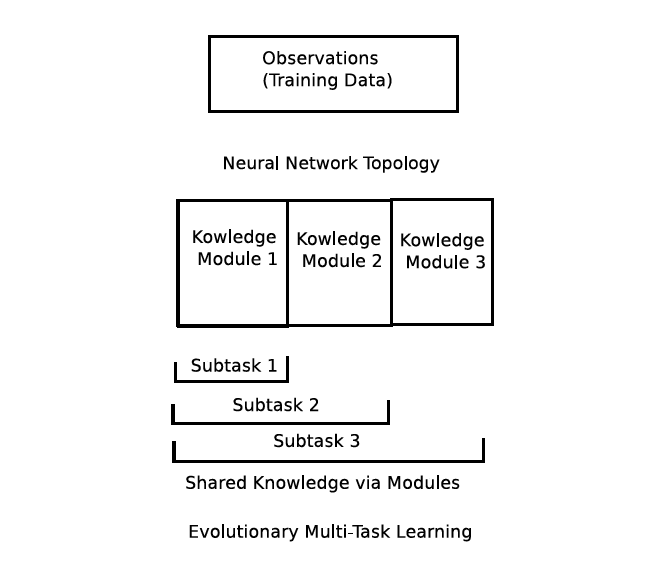
\includegraphics[width=1.2\linewidth]{images/modular.png}
            \caption{Mô hình biểu diễn mạng nơ-ron mô-đun hóa}
            \label{fig:problem:modular}
        \end{figure}
		\end{columns}
	\end{frame}
	
	\begin{frame}{Huấn luyện nhiều mạng Nơ-ron đa cấu trúc}
		\begin{itemize}
		    \begin{block}{Vấn đề}
		        \textcolor{red}{Khi cấu trúc mạng thay đổi không tận dụng được tri thức đã học từ cấu trúc mạng trước đó. Hoặc khi muốn tìm cấu trúc mạng tối ưu cho một bài toán.}
		    \end{block}
		    \begin{block}{Phát biểu bài toán}
		        \begin{itemize}
		            \item Cho $K$ tác vụ $T_1, T_2, ... T_K$ với $j \in [1,K]$.
		            \item Mỗi tác vụ tương đương với một bài toán tối ưu hóa 1 cấu trúc mạng nơ-ron lần lượt là $h_1, h_2, ... , h_K$ khác nhau.
		        \end{itemize}
		        Mục tiêu: \textcolor{red}{Khai thác mối quan hệ tiềm ẩn, tối ưu hóa đồng thời $K$ tác vụ.}
		    \end{block}
		\end{itemize}
	\end{frame}
	
	\begin{frame}{Giải thuật tiến hóa đề xuất}
	    \begin{itemize}
		    \begin{block}{Huấn luyện nhiều mạng nơ-ron có cấu trúc mô-đun}
		        \begin{enumerate}
		            \setlength\itemsep{0.01em}
		            \item Coi cấu trúc mạng được coi là một tác vụ tối ưu
		            \item Sử dụng thuật toán tiến hóa đa nhiệm MFEA-I, MFEA-II.
		            \item Đánh giá từng cá thể của tác vụ tương ứng với cấu trúc mạng nơ-ron của nó
		        \end{enumerate}
		        Vấn đề: \textcolor{red}{Mã hóa, giải mã từng cá thể để phù hợp với các cấu trúc mạng nơ-ron riêng biệt}
		    \end{block}
		    \begin{block}{Đề xuất}
		        \begin{enumerate}
		            \setlength\itemsep{0.01em}
		            \item Không gian biểu diễn chung cho các cấu trúc mạng kich thước $D$.
		            \item Thuật toán mã hóa, giải mã các cá thể:
		            \begin{itemize}
		                \setlength\itemsep{0.01em}
		                \item Mã hóa: Các tham số $(w,b)$ được mã hóa "gián tiếp" vào véc-tơ có kích thước $D$.
		                \item Giải mã: Từ cá thể có kích thước $D$ trả về bộ tham số $(w,b)$ tính giá trị hàm lỗi tương ứng.
		            \end{itemize}
		        \end{enumerate}
		    \end{block}
		\end{itemize}
	\end{frame}
	\begin{frame}{Mô tả thuật toán}
	    \begin{itemize}
		    \begin{block}{Giả định}
		        \begin{itemize}
	                \setlength\itemsep{0.01em}
	                \item Cho $K$ tác vụ $T_1, T_2, ... ,T_k$ với $j \in [1,K]$. Mỗi tác vụ tương đương với một mô hình mạng neural có số lượng lớp ẩn và số lượng nút tại lớp ẩn khác nhau. 
                    \item Định nghĩa $l_j$ là số lượng lớp trong cấu trúc mạng của tác vụ $T_j$, $h_j^{(i)}$ là số lượng nút tại lớp ẩn thứ i của tác vụ $T_j$ với  $j \in [1,K]$ và  $i \in [1,l_j]$.
                    % \item Định nghĩa $\theta = \max_{j \in [1,K]}l_j$ là số lượng lớp lớn nhất trong tất cả các tác vụ. Vậy $h_{multitask}^{\theta} = \max_{j \in [1,K]}h_j^{(l_j)}$ là số lượng nút lớn nhất ở lớp cuối cùng của tất cả các tác vụ. 
	            \end{itemize}
		    \end{block}
		    \begin{block}{Thuật toán}
		        \begin{enumerate}
		            \item Tính $H_{multitask}$ bao gồm tất cả các tham số của không gian tìm kiếm chung.
		            Khởi tạo không gian tìm kiếm chung với kích thước:\\
		            $D_{unified} = \sum_{l={1,...L}}h_{l-1}h_l + h_l$ từ ma trận $H_{multitask}$.
                    \item Khởi tạo $W_{multitask}$, Danh sách các ma trận trọng số tương ứng với $H_{multitask}$.
                    \item Tính $W_{j}$, tương ứng với ma trận trọng số $h_{j}$ với $j \in \{1, ..,K\}$
		        \end{enumerate}
		    \end{block}
		\end{itemize}
	\end{frame}
	
	\begin{frame}{Ví dụ}
	    \begin{block}{}
	        \textcolor{blue}{Bài toán: } Giả sử ta có 3 tác vụ có cấu trúc mạng tương ứng với $H_1 = [2, 2, 2, 1]$, $H_2 = [2, 3, 2, 1]$ và $H_3 = [2, 3, 1]$. Áp dụng thuật toán mã hóa, giải mã với các tác vụ này
	    \end{block}
	    \begin{block}{Tính $H_{multitask}$ và không gian biểu diễn chung}
	        \begin{columns}
	        \column{0.5\linewidth}
	        \begin{enumerate}
	            \setlength\itemsep{0.01em}
	            \item Tính $H_{multitask}$: $H_{multitask}=[2, 3, 3, 1]$ \Rightarrow Tổng số tham số: $D_{unified} = \sum_{l={1,...L}}h_{l-1}h_l + h_l$ \Rightarrow \textbf{25 tham số}.
	            \item Một kiểu gen (genotype) được biểu diễn dưới dạng:
	            \centerline{$
                  genotype=
                  \begin{bmatrix}
                    1& 2& 3& \dots & 25
                  \end{bmatrix}
                $}
	        \end{enumerate}
	        \column{0.5\linewidth}
	        \begin{figure}[]
                    \centering
                    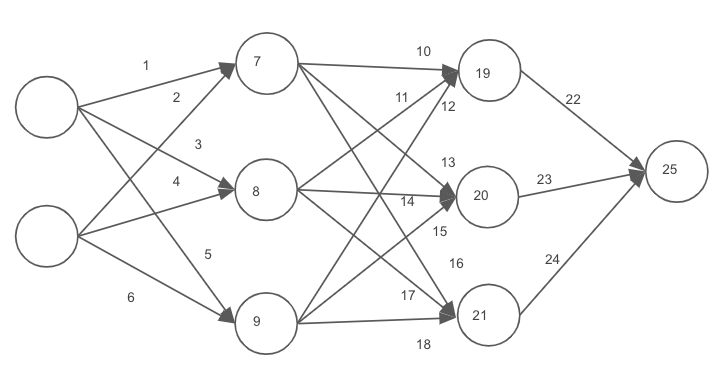
\includegraphics[width=1.0\linewidth]{images/neural-ex1.png}
                    \caption{Mạng Nơ-ron biểu diễn chung}
                    \label{fig:problem:neural-ex1}
            \end{figure}
	        \end{columns}
	    \end{block}
    \end{frame}
%     \begin{frame}{Ví dụ (2)}
% 		    \begin{block}{Bước 2: Tính danh sách ma trận trọng số: $W_{multitask}$}
% 		        \begin{columns}
% 		            \column{0.3\textwidth}
% 		            Lớp 1:
% 		            \begin{equation*}
% 		            \\
% 		              \begin{array}{l}
%                       W_1=
%                       \begin{bmatrix}
%                         1& 3& 5\\
%                         2& 4& 6
%                       \end{bmatrix}\\
%                       \\
%                       b_1=
%                       \begin{bmatrix}
%                         7& 8& 9
%                       \end{bmatrix}
%                     \end{array}

%                     \end{equation*}
                    
%                     \column{0.3\textwidth}
%                     Lớp 2:
%                     \begin{align*}
%                     \begin{array}{l}
%                       W_2=
%                       \begin{bmatrix}
%                         10& 13& 16\\
%                         11& 14& 17\\
%                         12& 15& 18
%                       \end{bmatrix}\\
%                       \\
%                       b_2=
%                       \begin{bmatrix}
%                         19& 20& 21\\
%                       \end{bmatrix}
%                       \end{array}
%                     \end{align*}
%                     \column{0.3\textwidth}
%                     Lớp 3:
%                     \begin{align*}
%                     \begin{array}{l}
%                       W_3=
%                       \begin{bmatrix}
%                         22\\
%                         23\\
%                         24
%                       \end{bmatrix}\\
%                       \\
%                       b_3=
%                       \begin{bmatrix}
%                         25
%                       \end{bmatrix}
%                       \end{array}
%                     \end{align*}
% 		        \end{columns}
% 		    \end{block}
% 	\end{frame}
% 	\begin{frame}{Bước 3: Giải mã bộ trọng số $W_j$, $b_j$ trên mỗi tác vụ}
%     		    \begin{columns}
%         		\column{0.3\textwidth}
%         		    \begin{block}{Task1: $H_1 = [2, 2, 2, 1]$}
%         		    \begin{equation*}
%         		      \begin{array}{l}
        		      
%                       W_1=
%                       \begin{bmatrix}
%                         1& 3\\
%                         2& 4
%                       \end{bmatrix},\\
%                       \\
%                       b_1=
%                       \begin{bmatrix}
%                         7& 8
%                       \end{bmatrix}
%                       \end{array}
%                     \end{equation*}
                
%                     \begin{equation*}
%                     \begin{array}{l}
%                       W_2=
%                       \begin{bmatrix}
%                         10& 13\\
%                         11& 14
%                       \end{bmatrix},\\
%                       \\
%                       b_2=
%                       \begin{bmatrix}
%                         19& 20\\
%                       \end{bmatrix}
%                       \end{array}
%                     \end{equation*}
%                     \begin{equation*}
%                     \begin{array}{l}
%                       W_3=
%                       \begin{bmatrix}
%                         22\\
%                         23
%                       \end{bmatrix},\\
%                       \\
%                       b_3=
%                       \begin{bmatrix}
%                         25
%                       \end{bmatrix}
%                       \end{array}
%                     \end{equation*}
%                 \end{block}
                    
%         	\column{0.3\textwidth}
%         		\begin{block}{Task2: $H_2 = [2, 3, 2, 1]$}
%                 \begin{equation*}
%                 \begin{array}{l}
%                   W_1=
%                   \begin{bmatrix}
%                     1& 3& 5\\
%                     2& 4& 6
%                   \end{bmatrix},\\
%                   \\
%                   b_1=
%                   \begin{bmatrix}
%                     7& 8& 9
%                   \end{bmatrix}
%                   \end{array}
%                 \end{equation*}
            
%                 \begin{equation*}
%                 \begin{array}{l}
%                   W_2=
%                   \begin{bmatrix}
%                     10& 13\\
%                     11& 14\\
%                     12& 15
%                   \end{bmatrix},\\
%                   \\
%                   b_2=
%                   \begin{bmatrix}
%                     19& 20\\
%                   \end{bmatrix}
%                   \end{array}
%                 \end{equation*}
            
            
%                 \begin{equation*}
%                 \begin{array}{l}
%                   W_3=
%                   \begin{bmatrix}
%                     22\\
%                     23
%                   \end{bmatrix},\\
%                   \\
%                   b_3=
%                   \begin{bmatrix}
%                     25
%                   \end{bmatrix}
%                   \end{array}
%                 \end{equation*}
%                 \end{block}
%         		\column{0.3\textwidth}
        		
%         		\begin{block}{Task3: $H_3 = [2, 3, 1]$}
%                 \begin{equation*}
%                 \begin{array}{l}
%                   W_1=
%                   \begin{bmatrix}
%                     1& 3& 5\\
%                     2& 4& 6
%                   \end{bmatrix},\\
%                   \\
%                   b_1=
%                   \begin{bmatrix}
%                     7& 8& 9
%                   \end{bmatrix}
%                   \end{array}
%                 \end{equation*}
            
%                 \begin{equation*}
%                 \begin{array}{l}
%                   W_2=
%                   \begin{bmatrix}
%                     22\\
%                     23\\
%                     24
%                   \end{bmatrix},\\
%                   \\
%                   b_2=
%                   \begin{bmatrix}
%                     25
%                   \end{bmatrix}
%                   \end{array}
%                 \end{equation*}
%                 \end{block}
%     		    \end{columns}
% 	\end{frame}
	\begin{frame}{Ví dụ: Trực quan các bước}
		\begin{figure}[h!] 
            \centering
            \fbox{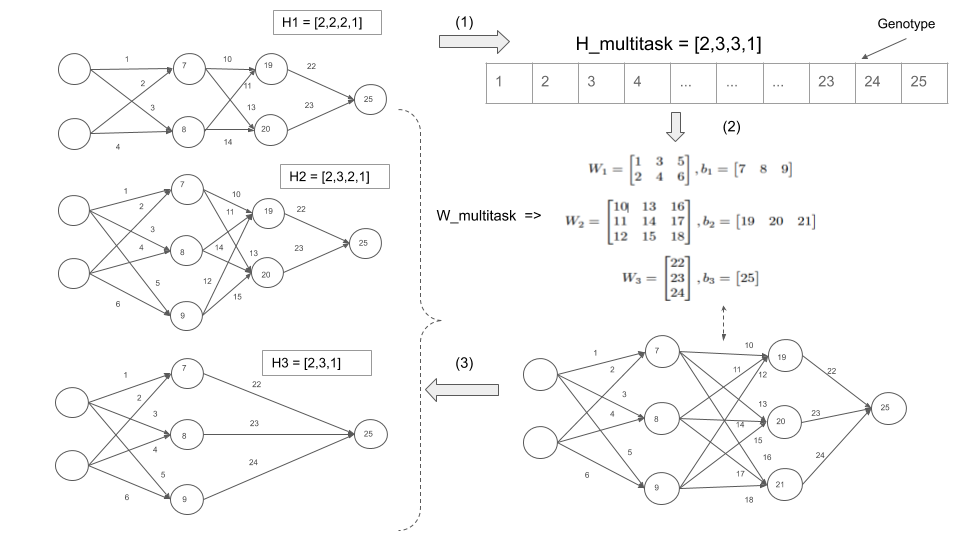
\includegraphics[width=1.0\linewidth, height=6cm]{images/modular-ex.png}}
            \caption{Ví dụ thuật toán đề xuất cho các mô hình mạng H1(2,2,2,1), H2(2,3,2,1), H3(2,3,1)}
            \label{fig:problem:modular-ex1}
        \end{figure}
	\end{frame}
	\begin{frame}{Mã hóa, giải mã cá thể}
	    \begin{figure}[]
            \centering
            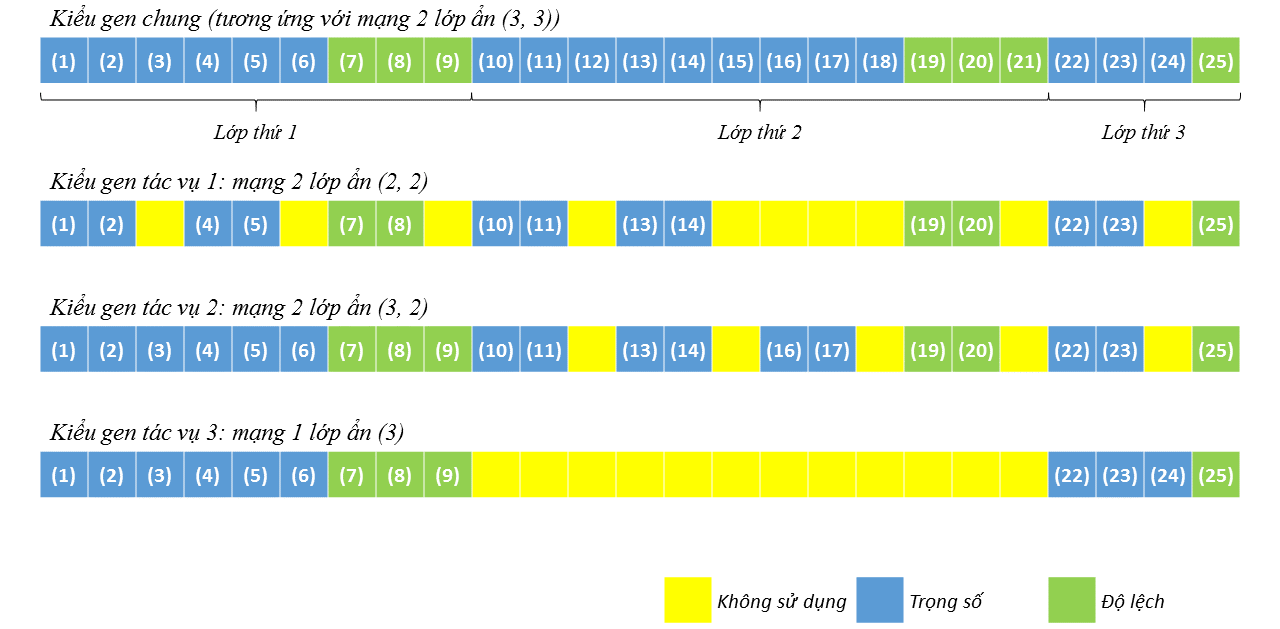
\includegraphics[width=1.0\linewidth]{images/neural-decode.jpg}
            \caption{Biểu diễn không gian chung và biểu diễn từng cá thể}
            \label{fig:problem:neural-ex1}
        \end{figure}
        \textit{Sử dụng phép lai ghép SBX, PMU thông thường, phù hợp với giả thiết parent-centric}.
	\end{frame}